\documentclass[tikz,border=3mm]{standalone}
\usetikzlibrary{shapes, positioning}
\begin{document}
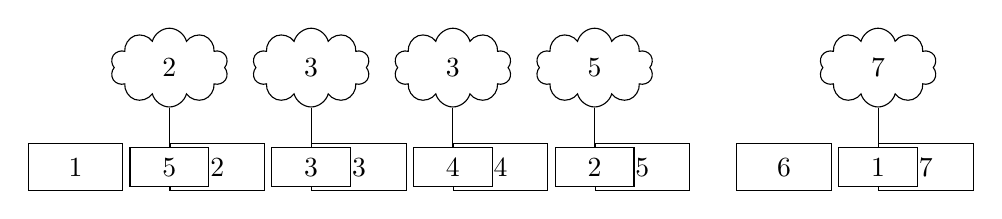
\begin{tikzpicture}[
    parkingspot/.style={draw, minimum width=1.2cm, minimum height=0.6cm, anchor=west},
    car/.style={draw, fill=white, minimum width=1cm, minimum height=0.5cm, align=center},
    thoughtbubble/.style={cloud, draw, cloud puffs=10, cloud ignores aspect, minimum width=1.5cm, minimum height=1cm, align=center}
]
% Draw parking spots 1 to 7
\foreach \i in {1,...,7} {
    \node[parkingspot] (spot\i) at (\i*1.8, 0) {\i};
}
% Place cars in their parked positions
\node[car] (car1) at (7*1.8, 0) {1};
\node[car] (car2) at (5*1.8, 0) {2};
\node[car] (car3) at (3*1.8, 0) {3};
\node[car] (car4) at (4*1.8, 0) {4};
\node[car] (car5) at (2*1.8, 0) {5};
% Add thought bubbles with preferred spots
\node[thoughtbubble, above=0.5cm of car1] (bubble1) {7};
\node[thoughtbubble, above=0.5cm of car2] (bubble2) {5};
\node[thoughtbubble, above=0.5cm of car3] (bubble3) {3};
\node[thoughtbubble, above=0.5cm of car4] (bubble4) {3};
\node[thoughtbubble, above=0.5cm of car5] (bubble5) {2};
% Connect cars to their thought bubbles
\foreach \i in {1,...,5} {
    \draw[-] (car\i) -- (bubble\i);
}
% Label original positions (already on cars) and preferred spots (in bubbles)
\end{tikzpicture}
\end{document}